\section{Results}\label{sec:results}
In order to be able to correctly analyse the diffraction pattern of a helix let us deconstruct it into segments.
Slit patterns can be thought of as an approximation of one-dimensional sections of a helix, they also have a well-known solution which we have confirmed by measuring the diffractions from those slit patterns.

\begin{figure}[H]
    \centering
    \begin{subfigure}{0.48\columnwidth}
        \centering
        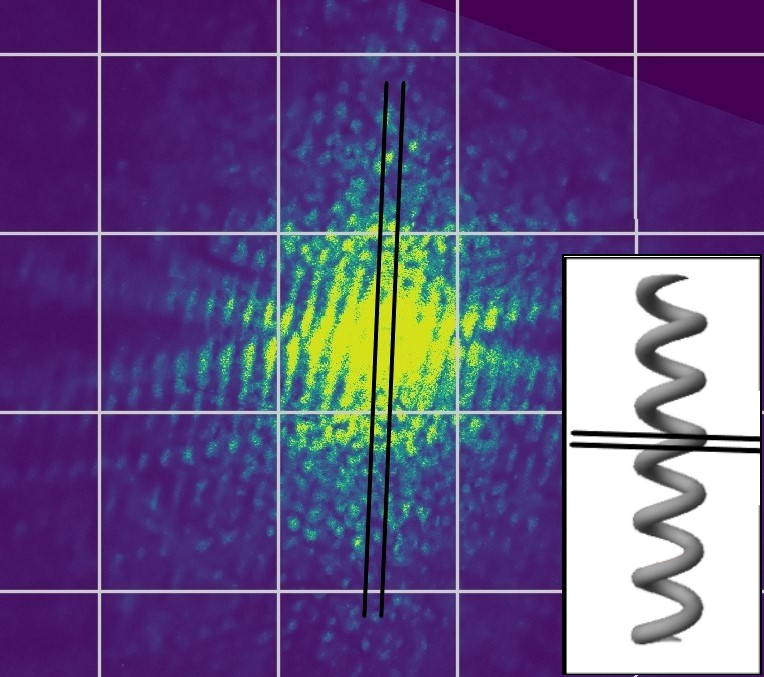
\includegraphics[width=\columnwidth]{figures/HelixSection2.png} % second figure itself
        \caption{Single slit section}
        \label{fig:HelixSection1}
    \end{subfigure}
    \begin{subfigure}{0.48\columnwidth}
        \centering
        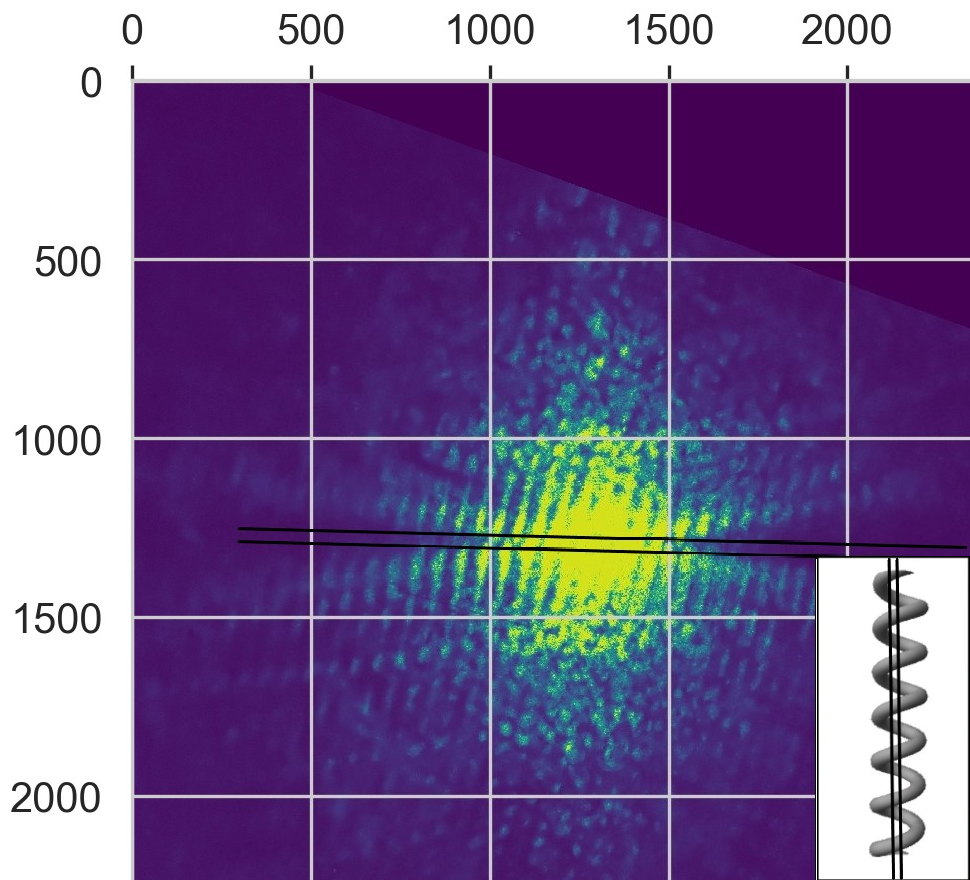
\includegraphics[width=\columnwidth]{figures/HelixSection1.png}
        \caption{N-slits section}
        \label{fig:HelixSection2}
    \end{subfigure}
    \begin{subfigure}{0.46\columnwidth}
        \centering
        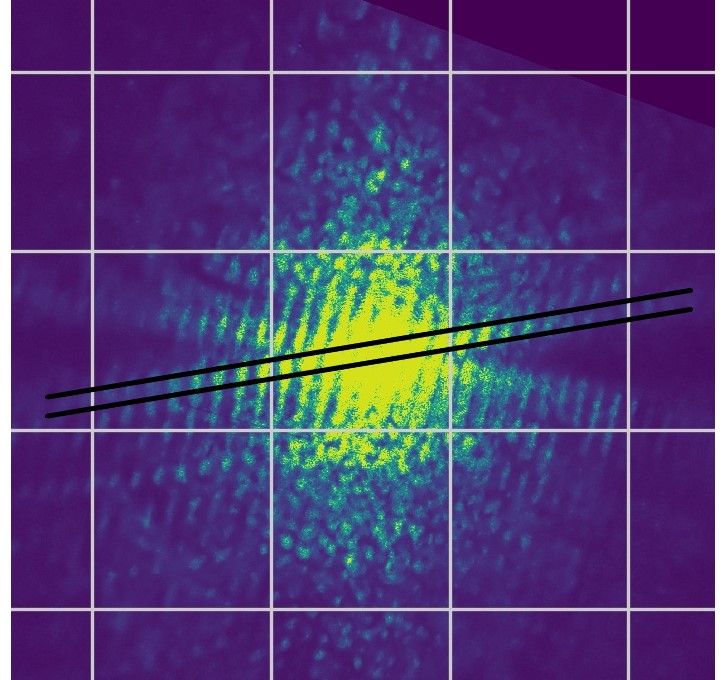
\includegraphics[width=\columnwidth]{figures/HelixSection4.jpg} % second figure itself
        \caption{"X" section 1}
        \label{fig:HelixSection3}
    \end{subfigure}
    \begin{subfigure}{0.48\columnwidth}
        \centering
        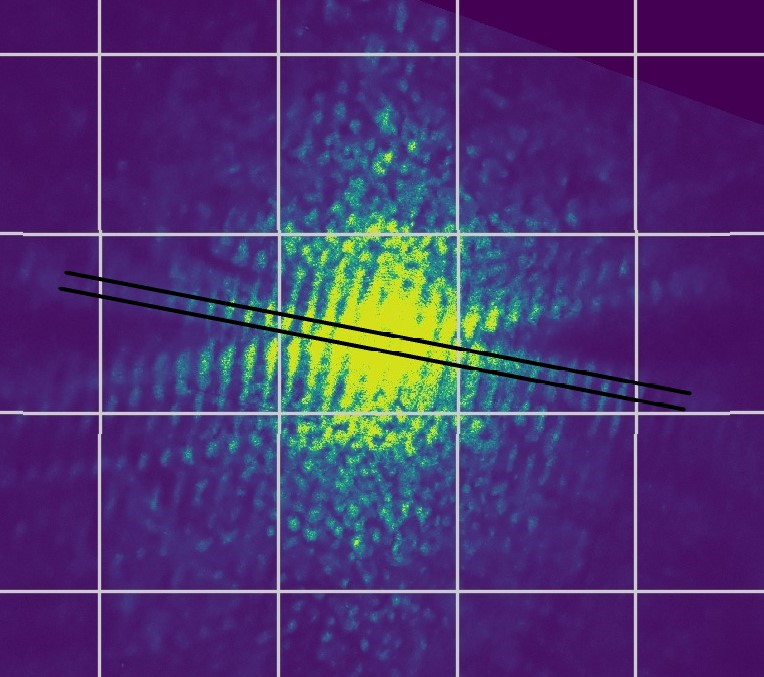
\includegraphics[width=\columnwidth]{figures/HelixSection3.jpg} % second figure itself
        \caption{"X" section 2}
        \label{fig:HelixSection4}
    \end{subfigure}
    \caption{Deconstruction of diffraction pattern to known 1D sections.}
    \label{fig:HelixSections}
\end{figure}

\subsection{Single slit section}
Taking the horizontal section of the helix we noticed that it can be described as:
\[T(x)\approx 1-rect(\frac{x}{2R})\]
Where we treat the helix as approximately a cylinder, which is, in the context of our 1-D section (\ref{fig:HelixSection1}), the complement diffracting body of a single slit.
\begin{figure}[H]
    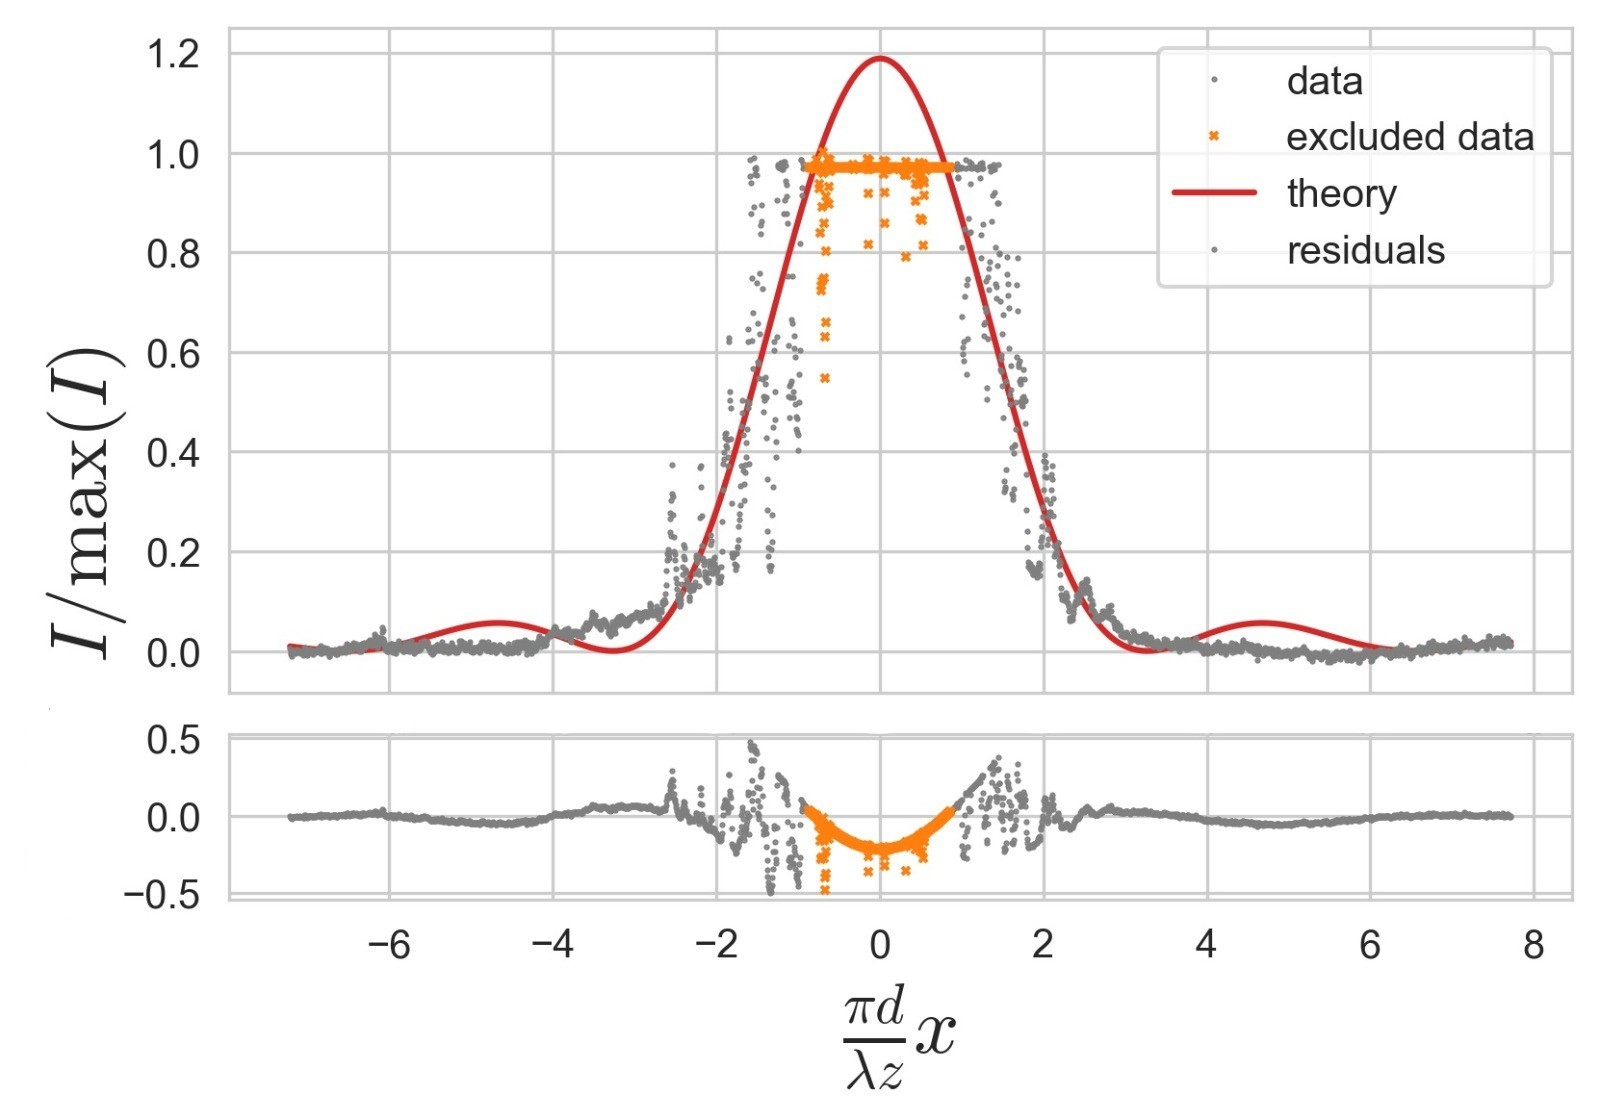
\includegraphics[width=0.9\columnwidth]{figures/Single slit section.jpeg}
    \caption{A fit for the single slit section of the helix using our model for single slit diffraction}
    \label{fig:Single slit section}
\end{figure}
The single slit model used in Figure~\ref{fig:Single slit section} describes the diffraction of our helix section with an error of $\sigma\approx0.1$.
The camera's sensor was saturated around $x=0$ and therefore that data was excluded from the fit.
We can also see oscillations around the main peak of the fit,

\subsection{N slits section}
If we take the section perpendicular to that we've discussed earlier, there's a resemblance to the n slits pattern.
The width of the helix is now the distance between two slits, and the pitch is the width of each slit.
For the section taken along the middle of the helix we have: \[L=\frac{p}{2}-d',d'=\frac{d}{\sin \theta}\]
Where $d'$ is the width of the effective slit.
\begin{figure}[H]
    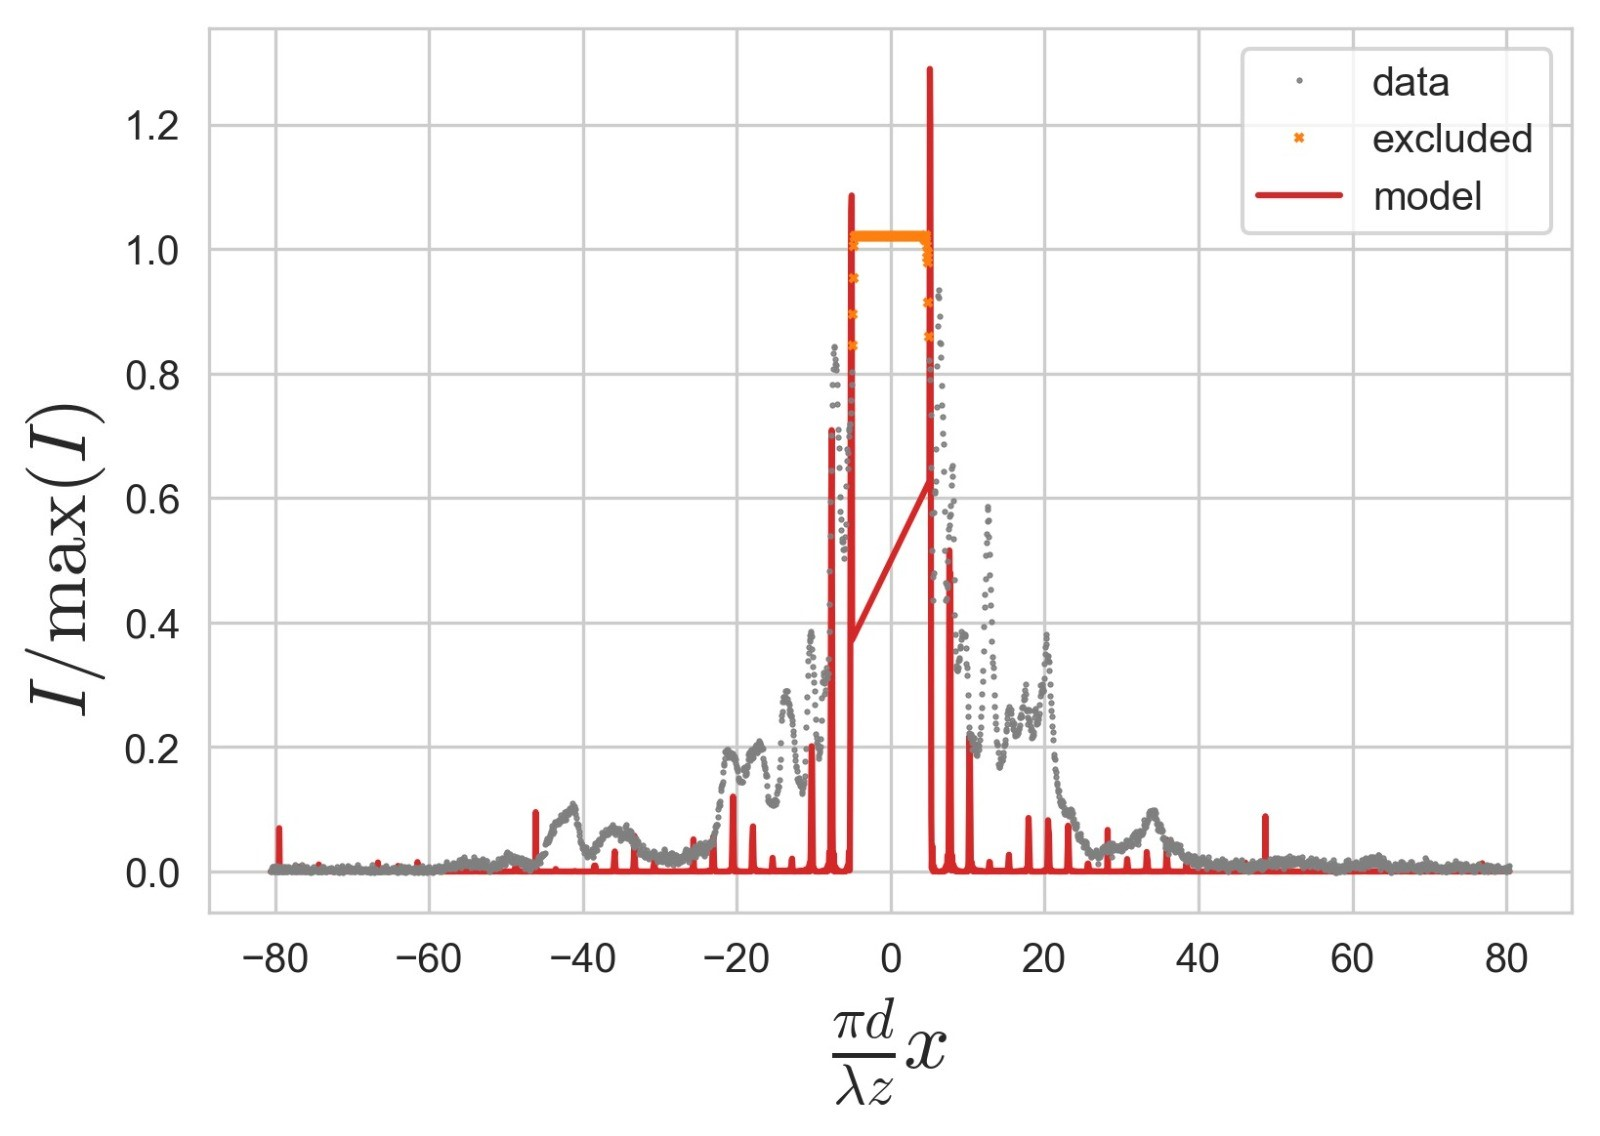
\includegraphics[width=0.9\columnwidth]{figures/n slits section.jpeg}
    \caption{A fit for the N-slits section using our model for N-slits diffraction}
    \label{fig:n slits section}
\end{figure}

\begin{figure}[H]
    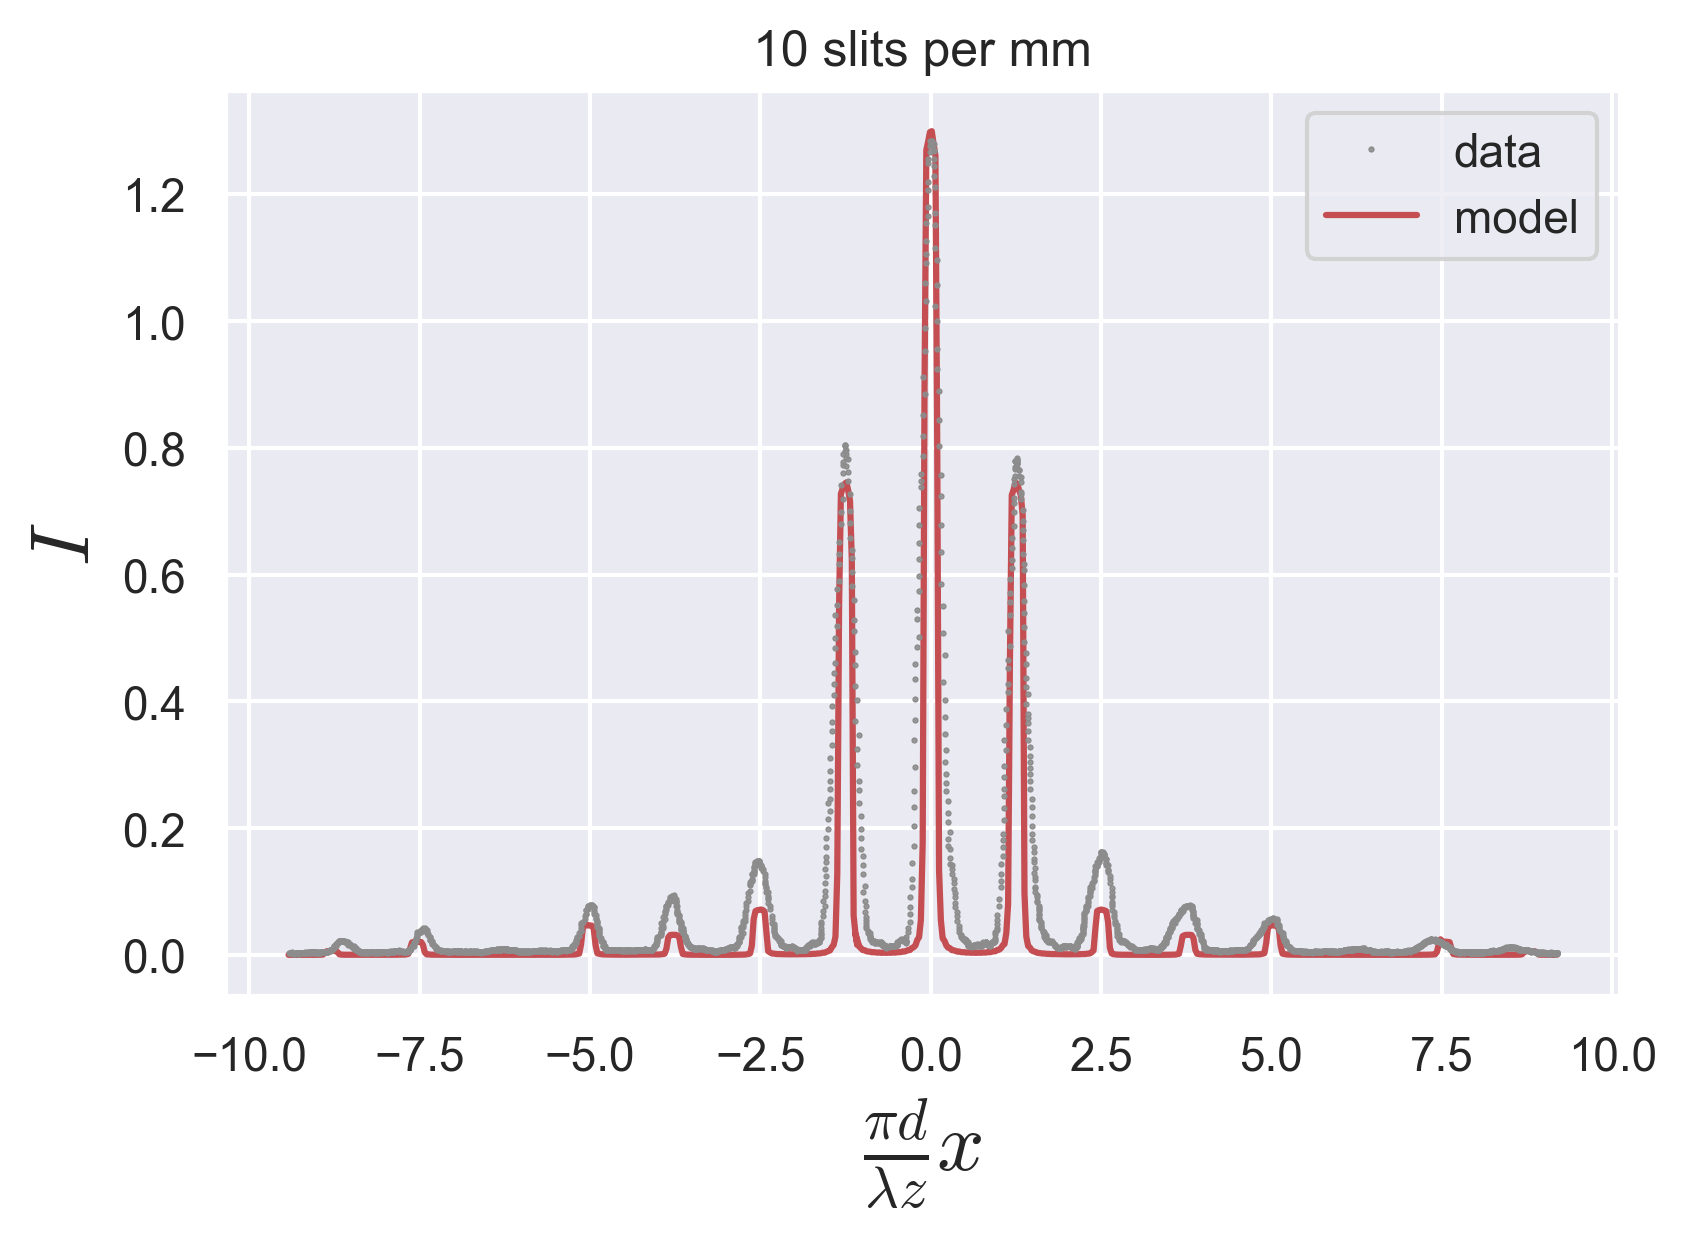
\includegraphics[width=0.9\columnwidth]{figures/10 slits per mm.png}
    \caption{}
    \label{fig:10 slits per mm}
\end{figure}
In the case of the periodic diffraction grating "10 lines per mm" the secondary effects are more pronounced especially
the photoelectric sensor's "memory" (The photoelectric sensor has a relaxation period in which to voltage diminishes
therefore after exposure instead of an immediate cut off a slope can be seen as the voltage is recorded with the relation
to the angle which continues to change during said period giving us higher peaks and wider slopes near those peaks)\\
\\
Finally To justify the title of the paper we should look at the interference pattern of the helix (Which bears some resemblance the shape off DNA)
according to equation \eqref{eq:farfield} and the specified approximations the interference pattern can be calculated using
the 2 dimensional fourier transform of the shape of the slit, Taking the inverse fourier transform of the pattern should result
In the square of the shape of the slit (since when calculating the intensity the square of $U$ was taken)
as can be shown by \ref{fig:expansion inverse fourie transform}
\begin{figure}[H]
    \centering
    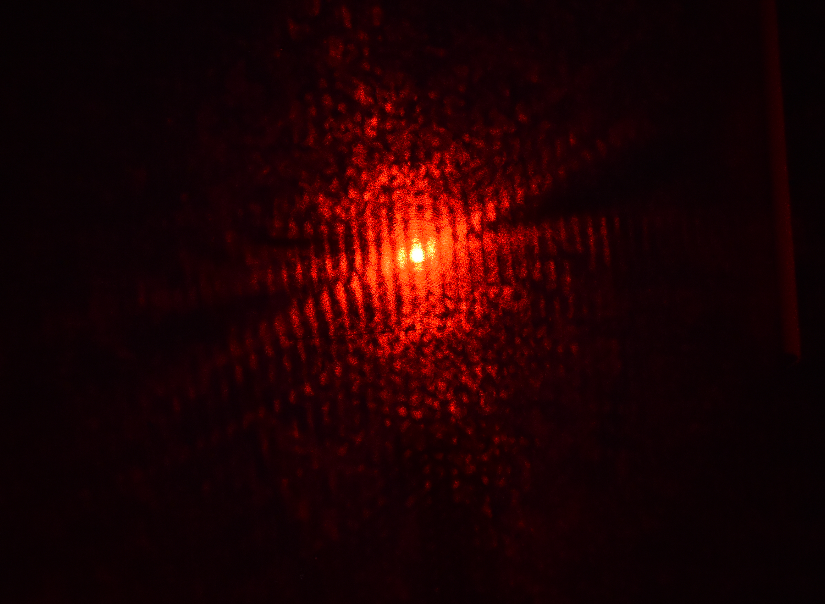
\includegraphics[width=0.9\columnwidth]{figures/expantion meshured interferemce.png}
    \caption{interference pattern measured as a result of diffraction with a helix}
    \label{fig:expansion measured interference pattern}
\end{figure}
\begin{figure}[H]
    \centering
    \begin{subfigure}{0.48\columnwidth}
        \centering
        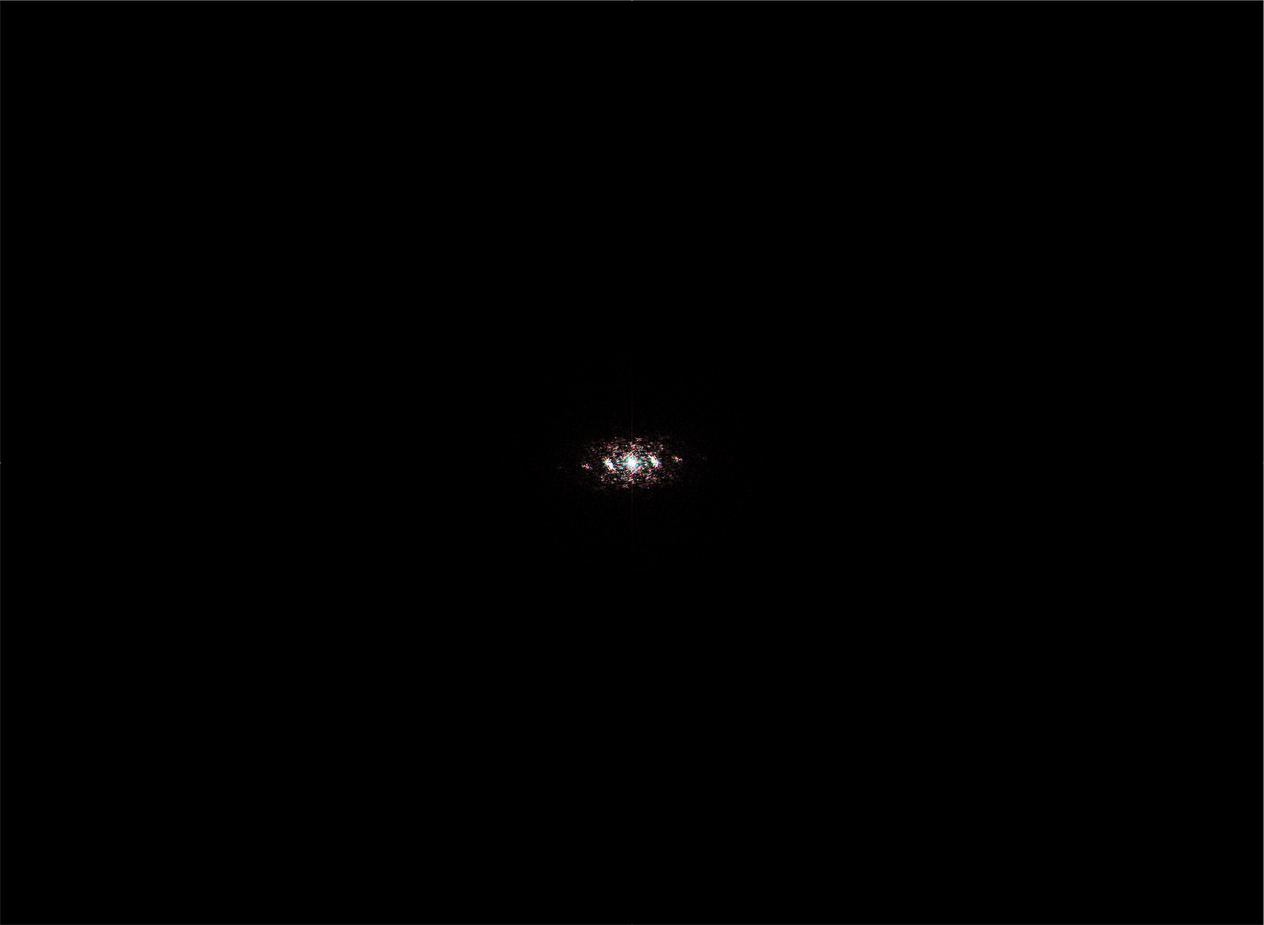
\includegraphics[width=0.9\columnwidth]{figures/expantion fourie transform.png}
        \caption{inverse discrete fourie transform calculated from the interference pattern at of the helix }
        \label{fig:expansion inverse fourie transform measured}
    \end{subfigure}\hfill
    \begin{subfigure}{0.48\columnwidth}
        \centering
        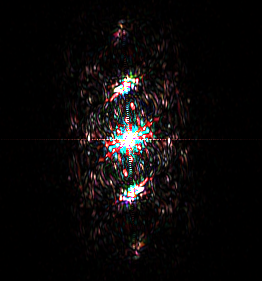
\includegraphics[width=\columnwidth]{figures/expantion fourie transform magnified.png} % second figure itself
        \caption{magnification of\ref{fig:expansion inverse fourie transform measured}}
        \label{fig:expansion fourie transform magnified}
    \end{subfigure}

    \label{fig:expansion theory measurements}
\end{figure}

As can be seen in \ref{fig:expansion fourie transform magnified} The result shows similarity to the calculation done in \ref{fig:expansion theory measurements}
in shape as in the orientation of the spring to the orientation of the "X"